\documentclass[12pt,a4paper]{extarticle}
\usepackage[margin=1in]{geometry}
\usepackage[slantfont,boldfont]{xeCJK}
\usepackage{graphicx}
\usepackage{caption}
\usepackage{float}
\usepackage{pgfplots}
\usepackage{subcaption}

\graphicspath{{./images/}}
\pgfplotsset{compat=1.12}
\setCJKmainfont{cwTeXKai}

\title{Machine Learning 2017 Spring\\Homework 4 Report}
\author{學號:\texttt{B03902048}\\系級:資工三\\姓名:林義聖}
\date{}

\begin{document}
\maketitle

\begin{itemize}

  \item[1.1] Dataset 中前 10 個人的前 10 張照片的平均臉和 PCA 得到的前 9 個 eigenfaces。
  \par 答:

  \begin{figure}[H]
    \begin{subfigure}[t]{0.5\textwidth}
      \centering
      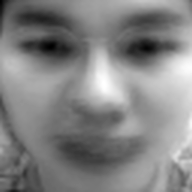
\includegraphics[width=0.8\linewidth]{average-face.png}
      \caption{The average face}
      \label{fig:average-face}
    \end{subfigure}
    \begin{subfigure}[t]{0.5\textwidth}
      \centering
      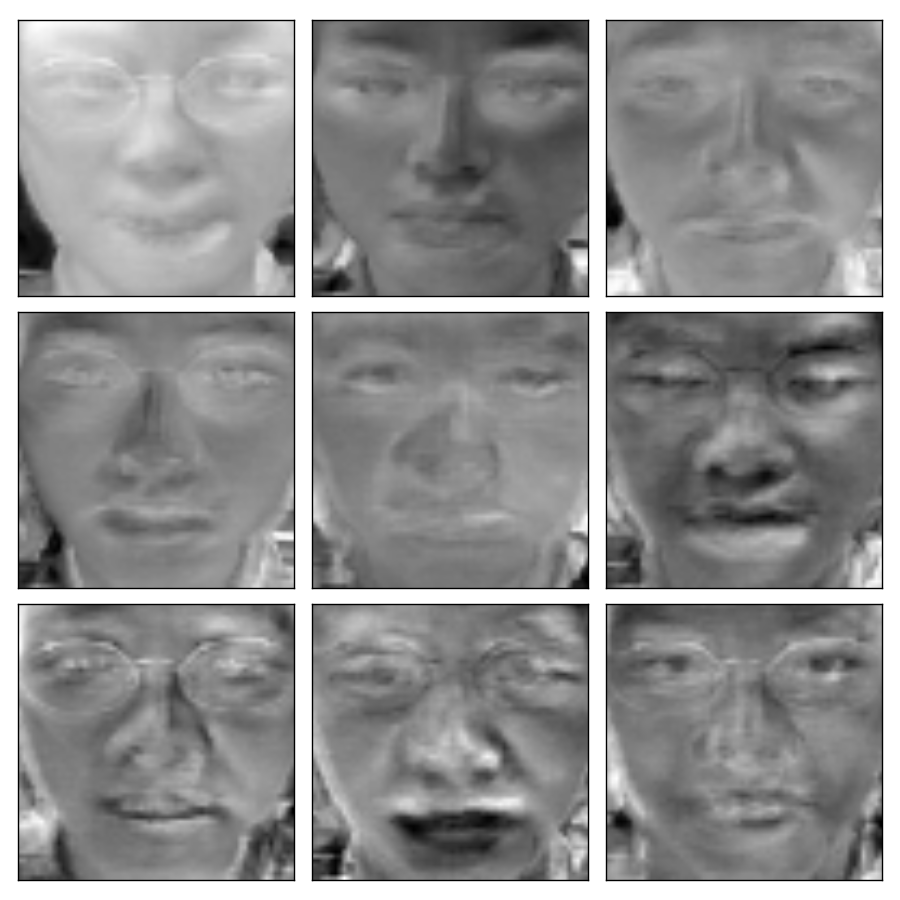
\includegraphics[width=0.8\linewidth]{eigen-faces-top-9.png}
      \caption{The top 9 eigenfaces}
      \label{fig:top-9-eigenfaces}
    \end{subfigure}
    \caption{}
  \end{figure}

  \item[1.2] Dataset 中前 10 個人的前 10 張照片的原始圖片和 reconstruct 圖(用前 5 個 eigenfaces)。
  \par 答:

  \begin{figure}[H]
    \begin{subfigure}[t]{0.5\textwidth}
      \centering
      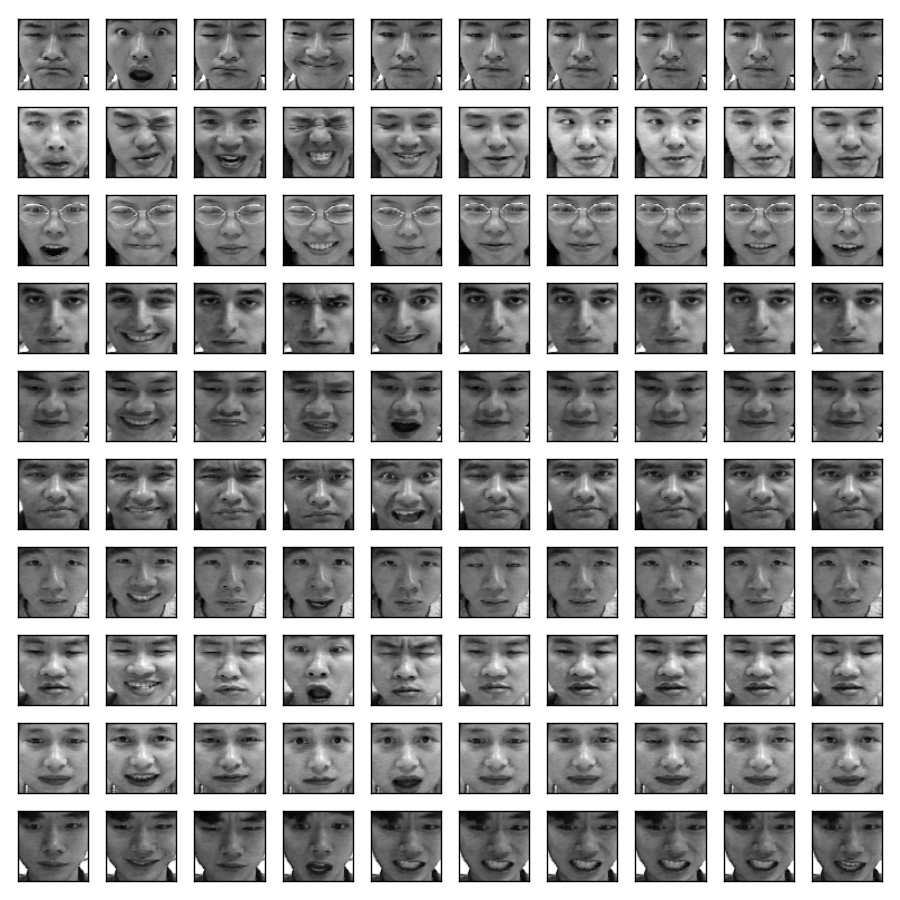
\includegraphics[width=\linewidth]{origin-faces-first-100.png}
      \caption{Original faces}
      \label{fig:original-faces}
    \end{subfigure}
    \begin{subfigure}[t]{0.5\textwidth}
      \centering
      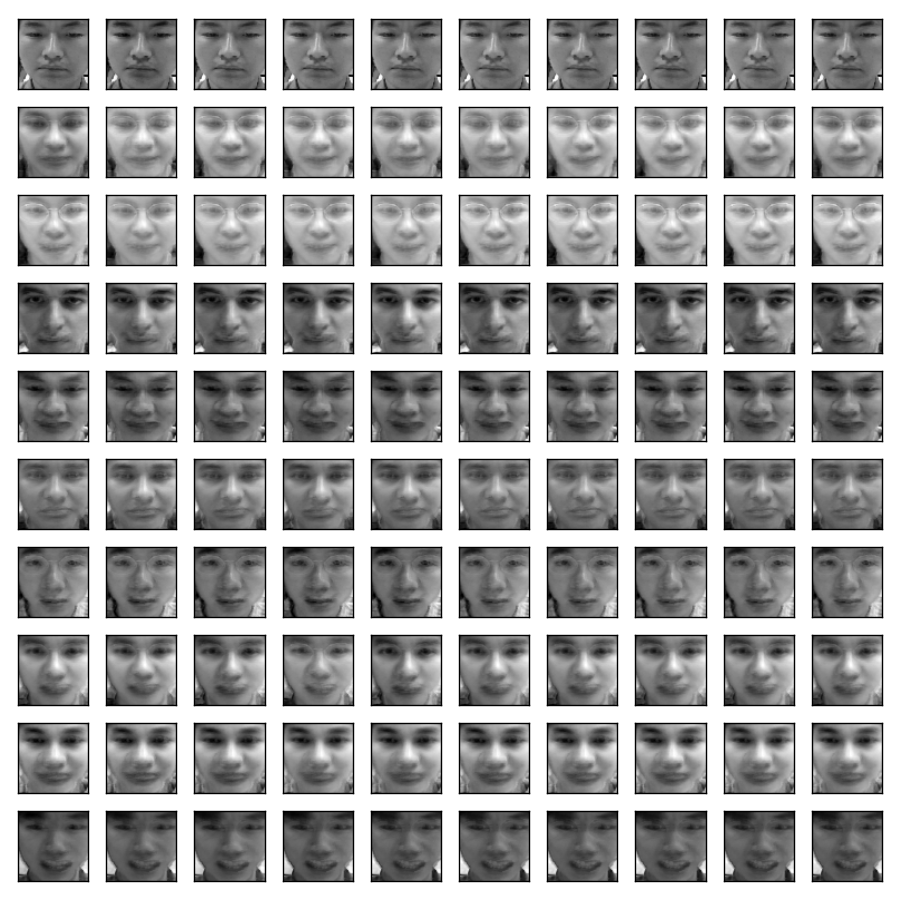
\includegraphics[width=\linewidth]{reconstruct-with-5-eigenfaces.png}
      \caption{Recovered faces}
      \label{fig:recovered-faces}
    \end{subfigure}
    \caption{100 faces reconstructed with top 5 eigenfaces}
    \label{fig:reconstruct-with-eigenfaces}
  \end{figure}

  \item[1.3] Dataset 中前 10 個人的前 10 張照片投影到 top $k$ eigenfaces 時就可以達到 < 1\% 的 reconstruction error?
  \par 答:當 $k = 59$ 時可以達到。

  \begin{figure}[H]
    \centering
    \begin{tikzpicture}
      \begin{axis}[
        ytick={0, 0.01, 0.02, 0.03, 0.04, 0.05, 0.06, 0.07, 0.08, 0.09, 0.1},
        xlabel = \# of eigenfaces,
        ymajorgrids]
      \addplot[color=blue] table [x=nb, y=rate, col sep=comma] {reconstruct-error.csv};
      \end{axis}
    \end{tikzpicture}
    \caption{Reconstruction error (RMSE)}
    \label{fig:eigenfaces-error-rate}
  \end{figure}

  \item[2.1] 使用 word2vec toolkit 的各個參數的值與其意義。
  \par 答:

  \item[2.2] 將 word2vec 的結果投影到 2 維的圖。
  \par 答:

  \item[2.3] 從上題視覺化的圖中觀察到了什麼?
  \par 答:

  \item[3.1] 請詳加解釋你估計原始維度的原理、合理性,這方法的通用性如何?
  \par 答:

  \item[3.2] 將你的方法做在 hand rotation sequence datatset 上得到什麼結果?合理嗎?請討論之。
  \par 答:

  % \begin{table}[ht]
  %   \centering
  %   \caption{Probability distribution}
  %   \label{tab:prob-distribution}
  %   \begin{tabular}{|c|c|c|c|c|c|c|c|}\hline
  %   \# & Angry & Disgust & Fear & Happy & Sad & Surprice & Neutral \\\hline
  %   Figure \ref{fig:train-image-2} & 0.06 & 0 & 0.07 & 0 & 0.87 & 0 & 0 \\\hline
  %   Figure \ref{fig:train-image-6} & 0 & 0 & 0.48 & 0 & 0.44 & 0 & 0.08 \\\hline
  %   \end{tabular}
  % \end{table}
\end{itemize}

\end{document}
